\documentclass[12pt]{article}
\usepackage{amsmath}
\usepackage{titlesec}
\usepackage{cite}
\usepackage{graphicx}
\usepackage{float}
\usepackage{caption}
\usepackage{helvet}
\renewcommand{\familydefault}{\sfdefault}
\usepackage{subcaption}
\usepackage{wrapfig}
\usepackage{todonotes}
\RequirePackage{filecontents} 
\usepackage[margin=0.5in]{geometry}
\usepackage{cleveref}
\date{}
\titleformat{\subsection}
  {\normalfont\fontsize{11}{17}\sffamily\bfseries\slshape}
  {\thesubsection}
  {1em}
  {}
  
\begin{filecontents*}{\jobname.bib}
@article{qsar,
  doi = {10.1021/jm049228d},
  url = {http://dx.doi.org/10.1021/jm049228d},
  year  = {2005},
  month = {mar},
  publisher = {American Chemical Society ({ACS})},
  volume = {48},
  number = {5},
  pages = {1638--1648},
  author = {Richard A. Lewis},
  title = {A General Method for Exploiting {QSAR} Models in Lead Optimization},
  journal = {Journal of Medicinal Chemistry}
}
@Article{hx,
  doi = {10.1073/pnas.1404213111},
  url = {http://dx.doi.org/10.1073/pnas.1404213111},
  year  = {2014},
  month = {oct},
  publisher = {Proceedings of the National Academy of Sciences},
  volume = {111},
  number = {45},
  pages = {15975--15980},
  author = {J. J. Skinner and W. Yu and E. K. Gichana and M. C. Baxa and J. R. Hinshaw and K. F. Freed and T. R. Sosnick},
  title = {Benchmarking all-atom simulations using hydrogen exchange},
  journal = {Proceedings of the National Academy of Sciences}
}
@article{4OBEcite,
  doi = {10.1073/pnas.1404639111},
  url = {http://dx.doi.org/10.1073/pnas.1404639111},
  year  = {2014},
  month = {jun},
  publisher = {Proceedings of the National Academy of Sciences},
  volume = {111},
  number = {24},
  pages = {8895--8900},
  author = {J. C. Hunter and D. Gurbani and S. B. Ficarro and M. A. Carrasco and S. M. Lim and H. G. Choi and T. Xie and J. A. Marto and Z. Chen and N. S. Gray and K. D. Westover},
  title = {In situ selectivity profiling and crystal structure of {SML}-8-73-1,  an active site inhibitor of oncogenic K-Ras G12C},
  journal = {Proceedings of the National Academy of Sciences}
}
@Article{rasblood,
   Author="Reuter, C. W.  and Morgan, M. A.  and Bergmann, L. ",
   Title="{{T}argeting the {R}as signaling pathway: a rational, mechanism-based treatment for hematologic malignancies?}",
   Journal="Blood",
   Year="2000",
   Volume="96",
   Number="5",
   Pages="1655--1669",
   Month="Sep"
}
@article{hdxms,
  doi = {10.1039/c0cs00113a},
  url = {http://dx.doi.org/10.1039/c0cs00113a},
  year  = {2011},
  publisher = {Royal Society of Chemistry ({RSC})},
  volume = {40},
  number = {3},
  pages = {1224},
  author = {Lars Konermann and Jingxi Pan and Yu-Hong Liu},
  title = {Hydrogen exchange mass spectrometry for studying protein structure and dynamics},
  journal = {Chem. Soc. Rev.}
}
@article{tethering,
  doi = {10.1073/pnas.97.17.9367},
  url = {http://dx.doi.org/10.1073/pnas.97.17.9367},
  year  = {2000},
  month = {aug},
  publisher = {Proceedings of the National Academy of Sciences},
  volume = {97},
  number = {17},
  pages = {9367--9372},
  author = {D. A. Erlanson and A. C. Braisted and D. R. Raphael and M. Randal and R. M. Stroud and E. M. Gordon and J. A. Wells},
  title = {Site-directed ligand discovery},
  journal = {Proceedings of the National Academy of Sciences}
}
@article{dockingrev,
  doi = {10.1016/s1367-5931(02)00339-3},
  url = {http://dx.doi.org/10.1016/S1367-5931(02)00339-3},
  year  = {2002},
  month = {aug},
  publisher = {Elsevier {BV}},
  volume = {6},
  number = {4},
  pages = {439--446},
  author = {Brian K Shoichet and Susan L McGovern and Binqing Wei and John J Irwin},
  title = {Lead discovery using molecular docking},
  journal = {Current Opinion in Chemical Biology}
}
@article{itcref,
  doi = {10.1016/s0959-440x(00)00248-7},
  url = {http://dx.doi.org/10.1016/S0959-440X(00)00248-7},
  year  = {2001},
  month = {sep},
  publisher = {Elsevier {BV}},
  volume = {11},
  number = {5},
  pages = {560--566},
  author = {Stephanie Leavitt and Ernesto Freire},
  title = {Direct measurement of protein binding energetics by isothermal titration calorimetry},
  journal = {Current Opinion in Structural Biology}
}
@article{blast,
  doi = {10.1016/s0022-2836(05)80360-2},
  url = {http://dx.doi.org/10.1016/S0022-2836(05)80360-2},
  year  = {1990},
  month = {oct},
  publisher = {Elsevier {BV}},
  volume = {215},
  number = {3},
  pages = {403--410},
  author = {Stephen F. Altschul and Warren Gish and Webb Miller and Eugene W. Myers and David J. Lipman},
  title = {Basic local alignment search tool},
  journal = {Journal of Molecular Biology}
}
@article{modeller,
  doi = {10.1006/jmbi.1993.1626},
  url = {http://dx.doi.org/10.1006/jmbi.1993.1626},
  year  = {1993},
  month = {dec},
  publisher = {Elsevier {BV}},
  volume = {234},
  number = {3},
  pages = {779--815},
  author = {Andrej {\v{S}}ali and Tom L. Blundell},
  title = {Comparative Protein Modelling by Satisfaction of Spatial Restraints},
  journal = {Journal of Molecular Biology}
}
@article{openmm,
  doi = {10.1021/ct300857j},
  url = {http://dx.doi.org/10.1021/ct300857j},
  year  = {2013},
  month = {jan},
  publisher = {American Chemical Society ({ACS})},
  volume = {9},
  number = {1},
  pages = {461--469},
  author = {Peter Eastman and Mark S. Friedrichs and John D. Chodera and Randall J. Radmer and Christopher M. Bruns and Joy P. Ku and Kyle A. Beauchamp and Thomas J. Lane and Lee-Ping Wang and Diwakar Shukla and Tony Tye and Mike Houston and Timo Stich and Christoph Klein and Michael R. Shirts and Vijay S. Pande},
  title = {{OpenMM} 4: A Reusable,  Extensible,  Hardware Independent Library for High Performance Molecular Simulation},
  journal = {J. Chem. Theory Comput.}
}
@article{shirts2008,
  doi = {10.1063/1.2978177},
  url = {http://dx.doi.org/10.1063/1.2978177},
  year  = {2008},
  publisher = {{AIP} Publishing},
  volume = {129},
  number = {12},
  pages = {124105},
  author = {Michael R. Shirts and John D. Chodera},
  title = {Statistically optimal analysis of samples from multiple equilibrium states},
  journal = {J. Chem. Phys.}
}
@book{liu,
  author = "Jun S. Liu",
  title = "Monte Carlo strategies in scientific computing",
  publisher = "Springer",
  year = "2001",
  ISBN = "0387952306"
}
@article{kyle,
  doi = {10.1021/ct200463m},
  url = {http://dx.doi.org/10.1021/ct200463m},
  year  = {2011},
  month = {oct},
  publisher = {American Chemical Society ({ACS})},
  volume = {7},
  number = {10},
  pages = {3412--3419},
  author = {Kyle A. Beauchamp and Gregory R. Bowman and Thomas J. Lane and Lutz Maibaum and Imran S. Haque and Vijay S. Pande},
  title = {{MSMBuilder}2: Modeling Conformational Dynamics on the Picosecond to Millisecond Scale},
  journal = {J. Chem. Theory Comput.}
}
@Article{rasgtp,
   Author="Pai, E. F.  and Krengel, U.  and Petsko, G. A.  and Goody, R. S.  and Kabsch, W.  and Wittinghofer, A. ",
   Title="{{R}efined crystal structure of the triphosphate conformation of {H}-ras p21 at 1.35 {A} resolution: implications for the mechanism of {G}{T}{P} hydrolysis}",
   Journal="EMBO J.",
   Year="1990",
   Volume="9",
   Number="8",
   Pages="2351--2359",
   Month="Aug"
}
@article{rasgdp,
  doi = {10.1016/0022-2836(91)90753-s},
  url = {http://dx.doi.org/10.1016/0022-2836(91)90753-S},
  year  = {1991},
  month = {feb},
  publisher = {Elsevier {BV}},
  volume = {217},
  number = {3},
  pages = {503--516},
  author = {Liang Tong and Abraham M. de Vos and Michael V. Milburn and Sung-Hou Kim},
  title = {Crystal structures at 2.2 {\{AA}} resolution of the catalytic domains of normal ras protein and an oncogenic mutant complexed with {GDP}},
  journal = {Journal of Molecular Biology}
}
@article{deshaw,
  doi = {10.1371/journal.pone.0032131},
  url = {http://dx.doi.org/10.1371/journal.pone.0032131},
  year  = {2012},
  month = {feb},
  publisher = {Public Library of Science ({PLoS})},
  volume = {7},
  number = {2},
  pages = {e32131},
  author = {Kresten Lindorff-Larsen and Paul Maragakis and Stefano Piana and Michael P. Eastwood and Ron O. Dror and David E. Shaw},
  editor = {Daniel J. Muller},
  title = {Systematic Validation of Protein Force Fields against Experimental Data},
  journal = {{PLoS} {ONE}}
}
@article{craik,
  doi = {10.1126/science.1169378},
  url = {http://dx.doi.org/10.1126/science.1169378},
  year  = {2009},
  month = {apr},
  publisher = {American Association for the Advancement of Science ({AAAS})},
  volume = {324},
  number = {5924},
  pages = {213--215},
  author = {G. M. Lee and C. S. Craik},
  title = {Trapping Moving Targets with Small Molecules},
  journal = {Science}
}
@article{mark,
  doi = {10.1016/s1093-3263(00)80091-1},
  url = {http://dx.doi.org/10.1016/S1093-3263(00)80091-1},
  year  = {2000},
  month = {jan},
  publisher = {Elsevier {BV}},
  volume = {18},
  number = {4-5},
  pages = {452--463},
  author = {John M. Barnard and Geoff M. Downs and Annette von Scholley-Pfab and Robert D. Brown},
  title = {Use of Markush structure analysis techniques for descriptor generation and clustering of large combinatorial libraries},
  journal = {Journal of Molecular Graphics and Modelling}
}
@article{pyla,
  doi = {10.1038/nrc3106},
  url = {http://dx.doi.org/10.1038/nrc3106},
  year  = {2011},
  month = {oct},
  publisher = {Nature Publishing Group},
  volume = {11},
  number = {11},
  pages = {761--774},
  author = {Yuliya Pylayeva-Gupta and Elda Grabocka and Dafna Bar-Sagi},
  title = {{RAS} oncogenes: weaving a tumorigenic web},
  journal = {Nat Rev Cancer}
}
@article{kitchen2004,
  doi = {10.1038/nrd1549},
  url = {http://dx.doi.org/10.1038/nrd1549},
  year  = {2004},
  month = {nov},
  publisher = {Nature Publishing Group},
  volume = {3},
  number = {11},
  pages = {935--949},
  author = {Douglas B. Kitchen and H{\'{e}}l{\`{e}}ne Decornez and John R. Furr and J\"{u}rgen Bajorath},
  title = {Docking and scoring in virtual screening for drug discovery: methods and applications},
  journal = {Nat Rev Drug Discov}
}
@article{lyubartsev1992,
  doi = {10.1063/1.462133},
  url = {http://dx.doi.org/10.1063/1.462133},
  year  = {1992},
  publisher = {{AIP} Publishing},
  volume = {96},
  number = {3},
  pages = {1776},
  author = {A. P. Lyubartsev and A. A. Martsinovski and S. V. Shevkunov and P. N. Vorontsov-Velyaminov},
  title = {New approach to Monte Carlo calculation of the free energy: Method of expanded ensembles},
  journal = {J. Chem. Phys.}
}
@article{warren2006,
  doi = {10.1021/jm050362n},
  url = {http://dx.doi.org/10.1021/jm050362n},
  year  = {2006},
  month = {oct},
  publisher = {American Chemical Society ({ACS})},
  volume = {49},
  number = {20},
  pages = {5912--5931},
  author = {Gregory L. Warren and C. Webster Andrews and Anna-Maria Capelli and Brian Clarke and Judith LaLonde and Millard H. Lambert and Mika Lindvall and Neysa Nevins and Simon F. Semus and Stefan Senger and Giovanna Tedesco and Ian D. Wall and James M. Woolven and Catherine E. Peishoff and Martha S. Head},
  title = {A Critical Assessment of Docking Programs and Scoring Functions},
  journal = {Journal of Medicinal Chemistry}
}
@article{kuntz1999,
  doi = {10.1073/pnas.96.18.9997},
  url = {http://dx.doi.org/10.1073/pnas.96.18.9997},
  year  = {1999},
  month = {aug},
  publisher = {Proceedings of the National Academy of Sciences},
  volume = {96},
  number = {18},
  pages = {9997--10002},
  author = {I. D. Kuntz and K. Chen and K. A. Sharp and P. A. Kollman},
  title = {The maximal affinity of ligands},
  journal = {Proceedings of the National Academy of Sciences}
}
@article{perez2013,
  doi = {10.1063/1.4811489},
  url = {http://dx.doi.org/10.1063/1.4811489},
  year  = {2013},
  publisher = {{AIP} Publishing},
  volume = {139},
  number = {1},
  pages = {015102},
  author = {Guillermo Perez-Hernandez and Fabian Paul and Toni Giorgino and Gianni De Fabritiis and Frank Noe},
  title = {Identification of slow molecular order parameters for Markov model construction},
  journal = {J. Chem. Phys.}
}
@article{boresch2013,
  doi = {10.1021/jp0217839},
  url = {http://dx.doi.org/10.1021/jp0217839},
  year  = {2003},
  month = {sep},
  publisher = {American Chemical Society ({ACS})},
  volume = {107},
  number = {35},
  pages = {9535--9551},
  author = {Stefan Boresch and Franz Tettinger and Martin Leitgeb and Martin Karplus},
  title = {Absolute Binding Free Energies:~ A Quantitative Approach for Their Calculation},
  journal = {J. Phys. Chem. B}
}
@article{mak2014,
  doi = {10.1016/j.cllc.2014.09.005},
  url = {http://dx.doi.org/10.1016/j.cllc.2014.09.005},
  year  = {2014},
  month = {sep},
  publisher = {Elsevier {BV}},
  author = {Raymond H. Mak and Gretchen Hermann and John H. Lewis and Hugo J.W.L. Aerts and Elizabeth H. Baldini and Aileen B. Chen and Yolonda L. Colson and Fred H. Hacker and David Kozono and Jon O. Wee and Yu-Hui Chen and Paul J. Catalano and Kwok-Kin Wong and David J. Sher},
  title = {Outcomes by Tumor Histology and {KRAS} Mutation Status after Lung Stereotactic Body Radiation Therapy for Early Stage Non-Small Cell Lung Cancer},
  journal = {Clinical Lung Cancer}
}
@article{pi3k,
  doi = {10.1016/s0092-8674(00)00196-3},
  url = {http://dx.doi.org/10.1016/S0092-8674(00)00196-3},
  year  = {2000},
  month = {dec},
  publisher = {Elsevier {BV}},
  volume = {103},
  number = {6},
  pages = {931--944},
  author = {Michael E. Pacold and Sabine Suire and Olga Perisic and Samuel Lara-Gonzalez and Colin T. Davis and Edward H. Walker and Phillip T. Hawkins and Len Stephens and John F. Eccleston and Roger L. Williams},
  title = {Crystal Structure and Functional Analysis of Ras Binding to Its Effector Phosphoinositide 3-Kinase $\upgamma$},
  journal = {Cell}
}
@article{chodera,
  doi = {10.1063/1.3660669},
  url = {http://dx.doi.org/10.1063/1.3660669},
  year  = {2011},
  publisher = {{AIP} Publishing},
  volume = {135},
  number = {19},
  pages = {194110},
  author = {John D. Chodera and Michael R. Shirts},
  title = {Replica exchange and expanded ensemble simulations as Gibbs sampling: Simple improvements for enhanced mixing},
  journal = {J. Chem. Phys.}
}
@article{trpmut,
  doi = {10.1021/bi00098a002},
  url = {http://dx.doi.org/10.1021/bi00098a002},
  year  = {1991},
  month = {aug},
  publisher = {American Chemical Society ({ACS})},
  volume = {30},
  number = {34},
  pages = {8287--8295},
  author = {Bruno Antonny and Pierre Chardin and Michel Roux and Marc Chabre},
  title = {{GTP} hydrolysis mechanisms in ras p21 and in the ras-{GAP} complex studied by fluorescence measurements on tryptophan mutants},
  journal = {Biochemistry}
}
@article{chodera2014,
  doi = {10.1016/j.sbi.2014.04.002},
  url = {http://dx.doi.org/10.1016/j.sbi.2014.04.002},
  year  = {2014},
  month = {apr},
  publisher = {Elsevier {BV}},
  volume = {25},
  pages = {135--144},
  author = {John D Chodera and Frank No{\'{e}}},
  title = {Markov state models of biomolecular conformational dynamics},
  journal = {Current Opinion in Structural Biology}
}
@article{irwin2012,
  doi = {10.1021/ci3001277},
  url = {http://dx.doi.org/10.1021/ci3001277},
  year  = {2012},
  month = {jul},
  publisher = {American Chemical Society ({ACS})},
  volume = {52},
  number = {7},
  pages = {1757--1768},
  author = {John J. Irwin and Teague Sterling and Michael M. Mysinger and Erin S. Bolstad and Ryan G. Coleman},
  title = {{ZINC}: A Free Tool to Discover Chemistry for Biology},
  journal = {Journal of Chemical Information and Modeling}
}
@article{ostrem2013,
  doi = {10.1038/nature12796},
  url = {http://dx.doi.org/10.1038/nature12796},
  year  = {2013},
  month = {nov},
  publisher = {Nature Publishing Group},
  volume = {503},
  number = {7477},
  pages = {548--551},
  author = {Jonathan M. Ostrem and Ulf Peters and Martin L. Sos and James A. Wells and Kevan M. Shokat},
  title = {K-Ras(G12C) inhibitors allosterically control {GTP} affinity and effector interactions},
  journal = {Nature}
}
@article{bowman2012,
  doi = {10.1073/pnas.1209309109},
  url = {http://dx.doi.org/10.1073/pnas.1209309109},
  year  = {2012},
  month = {jul},
  publisher = {Proceedings of the National Academy of Sciences},
  volume = {109},
  number = {29},
  pages = {11681--11686},
  author = {G. R. Bowman and P. L. Geissler},
  title = {Equilibrium fluctuations of a single folded protein reveal a multitude of potential cryptic allosteric sites},
  journal = {Proceedings of the National Academy of Sciences}
}
@article{hendlich1997,
  doi = {10.1016/s1093-3263(98)00002-3},
  url = {http://dx.doi.org/10.1016/S1093-3263(98)00002-3},
  year  = {1997},
  month = {dec},
  publisher = {Elsevier {BV}},
  volume = {15},
  number = {6},
  pages = {359--363},
  author = {Manfred Hendlich and Friedrich Rippmann and Gerhard Barnickel},
  title = {{LIGSITE}: automatic and efficient detection of potential small molecule-binding sites in proteins},
  journal = {Journal of Molecular Graphics and Modelling}
}
@article{sun2012,
  doi = {10.1002/anie.201201358},
  url = {http://dx.doi.org/10.1002/anie.201201358},
  year  = {2012},
  month = {may},
  publisher = {Wiley-Blackwell},
  volume = {51},
  number = {25},
  pages = {6140--6143},
  author = {Qi Sun and Jason P. Burke and Jason Phan and Michael C. Burns and Edward T. Olejniczak and Alex G. Waterson and Taekyu Lee and Olivia W. Rossanese and Stephen W. Fesik},
  title = {Discovery of Small Molecules that Bind to K-Ras and Inhibit Sos-Mediated Activation},
  journal = {Angew. Chem. Int. Ed.}
}
@article{gilson1997,
  doi = {10.1016/s0006-3495(97)78756-3},
  url = {http://dx.doi.org/10.1016/S0006-3495(97)78756-3},
  year  = {1997},
  month = {mar},
  publisher = {Elsevier {BV}},
  volume = {72},
  number = {3},
  pages = {1047--1069},
  author = {M.K. Gilson and J.A. Given and B.L. Bush and J.A. McCammon},
  title = {The statistical-thermodynamic basis for computation of binding affinities: a critical review},
  journal = {Biophysical Journal}
}
@article{mobley2008,
  doi = {10.1021/jp0764384},
  url = {http://dx.doi.org/10.1021/jp0764384},
  year  = {2008},
  month = {jan},
  publisher = {American Chemical Society ({ACS})},
  volume = {112},
  number = {3},
  pages = {938--946},
  author = {David L. Mobley and Ken A. Dill and John D. Chodera},
  title = {Treating Entropy and Conformational Changes in Implicit Solvent Simulations of Small Molecules},
  journal = {J. Phys. Chem. B}
}
@article{nilmeier2011,
  doi = {10.1073/pnas.1106094108},
  url = {http://dx.doi.org/10.1073/pnas.1106094108},
  year  = {2011},
  month = {oct},
  publisher = {Proceedings of the National Academy of Sciences},
  volume = {108},
  number = {45},
  pages = {E1009--E1018},
  author = {J. P. Nilmeier and G. E. Crooks and D. D. L. Minh and J. D. Chodera},
  title = {Nonequilibrium candidate Monte Carlo is an efficient tool for equilibrium simulation},
  journal = {Proceedings of the National Academy of Sciences}
}
@article{drinkwater2010,
  doi = {10.1042/bj20100651},
  url = {http://dx.doi.org/10.1042/BJ20100651},
  year  = {2010},
  month = {sep},
  publisher = {Portland Press Ltd.},
  volume = {431},
  number = {1},
  pages = {51--61},
  author = {Nyssa Drinkwater and Hoan Vu and Kimberly~M. Lovell and Kevin~R. Criscione and Brett~M. Collins and Thomas~E. Prisinzano and Sally?Ann Poulsen and Michael~J. McLeish and Gary~L. Grunewald and Jennifer~L. Martin},
  title = {Fragment-based screening by X-ray crystallography,  {MS} and isothermal titration calorimetry to identify {PNMT} (phenylethanolamine N-methyltransferase) inhibitors},
  journal = {Biochem. J.}
}
@article{antan2014,
  doi = {10.1007/s10858-014-9848-9},
  url = {http://dx.doi.org/10.1007/s10858-014-9848-9},
  year  = {2014},
  month = {jul},
  publisher = {Springer Science $\mathplus$ Business Media},
  volume = {60},
  number = {1},
  pages = {37--44},
  author = {Aleksandar Antanasijevic and Benjamin Ramirez and Michael Caffrey},
  title = {Comparison of the sensitivities of {WaterLOGSY} and saturation transfer difference {NMR} experiments},
  journal = {J Biomol {NMR}}
}
@article{fesik,
  doi = {10.1002/anie.201201358},
  url = {http://dx.doi.org/10.1002/anie.201201358},
  year  = {2012},
  month = {may},
  publisher = {Wiley-Blackwell},
  volume = {51},
  number = {25},
  pages = {6140--6143},
  author = {Qi Sun and Jason P. Burke and Jason Phan and Michael C. Burns and Edward T. Olejniczak and Alex G. Waterson and Taekyu Lee and Olivia W. Rossanese and Stephen W. Fesik},
  title = {Discovery of Small Molecules that Bind to K-Ras and Inhibit Sos-Mediated Activation},
  journal = {Angew. Chem. Int. Ed.}
}
@article{chemtransform,
  doi = {10.1021/ci200379p},
  url = {http://dx.doi.org/10.1021/ci200379p},
  year  = {2011},
  month = {dec},
  publisher = {American Chemical Society ({ACS})},
  volume = {51},
  number = {12},
  pages = {3093--3098},
  author = {Markus Hartenfeller and Martin Eberle and Peter Meier and Cristina Nieto-Oberhuber and Karl-Heinz Altmann and Gisbert Schneider and Edgar Jacoby and Steffen Renner},
  title = {A Collection of Robust Organic Synthesis Reactions for In Silico Molecule Design},
  journal = {Journal of Chemical Information and Modeling}
}
\end{filecontents*}

\begin{document}

\section*{Specific Aims}
Ras family proteins, important in the control of cell growth, are commonly mutated in human cancer \cite{pyla}. Furthermore, mutations in Ras are also a leading cause of resistance to modern targeted therapy, and patients who harbor Ras mutations have considerably poorer prognoses than those with wild type Ras \cite{mak2014}. Targeting Ras has proven difficult, however, as its oncogenic mutants activate Ras primarily by inactivating its enzymatic activity, leaving inhibition of the enzyme an unworkable strategy. Further, the high affinity of GTP for Ras, resulting in the active Ras-GTP complex, combined with its high intracellular concentration renders outcompeting the bound nucleotide extremely difficult \cite{ostrem2013}. While recent experimental approaches have seen some success in identifying allosteric modulators \cite{ostrem2013}, these inhibitors are of limited application as they are currently of low affinity and therefore require the presence of a cysteine for covalent attachment \cite{ostrem2013}, present in only a small fraction of cancers. Worse still, this need for a cysteine results in a straightforward path to drug resistance. Here, we propose a novel strategy to design noncovalent ligands that allosterically inhibit Ras, using computational strategies where structural biology cannot elucidate hidden conformers.
\subsection*{Aim 1: Computationally map conformations accessible to Ras along with their corresponding energetics to identify potential opportunities for allosteric modulation}
We will first \textbf{identify metastable conformations and the associated energetics of oncogenic K-Ras using Markov State Model approaches}. Then, we intend to \textbf{mine the metastable conformations identified previously for potential ligand binding sites}. Following that analysis, we will \textbf{analyze the metastable conformations for putatively inactive conformations by comparison to other structures}. Finally, we will \textbf{develop fluorescence-based experimental assays to validate the conformational populations that we observed}.
 \subsection*{Aim 2: Identify new small molecule ligands of Ras}
 We will \textbf{perform virtual screening on a library of commercially-available compounds against putative allosteric binding sites}. Following that, we intend to \textbf{filter hits using free energy calculations}.  Finally, we will  \textbf{develop and validate a fluorescence-based assay for measuring weak allosteric binding and experimentally measure quantitative binding affinities of promising hits}. Finally, \textbf{we will computationally optimize derivatives of weak-binding scaffolds}, including existing scaffolds and those discovered in Aim 2 \textbf{using a new chemical Monte Carlo algorithm based on the method of expanded ensembles to search over large spaces of possible derivative molecules.} We will then \textbf{experimentally validate our derivatized ligands} to more tightly bind K-Ras.
 
 \subsection*{Conclusion}
   Having completed the above aims, our results will consist of novel chemical structures for targeting Ras, a novel computational pipeline for the discovery of allosteric sites and inhibitors, as well as insight into the conformational populations of a key signaling protein. 
  
  
  
  
  
  
  
 \clearpage


\section*{Innovation}
In this proposal, we develop a novel strategy for the design of allosteric ligands, and apply this strategy to the "undruggable" oncoprotein K-Ras. Taking advantage of recent advances in massively-parallel molecular simulation, we propose to use the developing field of Markov State Modeling to enumerate metastable conformations of K-Ras, giving unprecedented insight into both its functional dynamics and opportunities for its inhibition. We then develop a novel technique for exploring the relevant chemical space in ligand design for identified binding sites, allowing us to use physical principles to examine the structure-activity relationship of ligand binding to these previously undiscovered sites. We also propose to experimentally validate these techniques, providing a guide for the future examination of Ras allosteric ligands experimentally.

\underline{Expanded-ensemble simulation to explore chemical space.} We will use the technique of expanded-ensemble simulation \cite{lyubartsev1992} over chemical space, with an appropriate bias, to guide the simulation toward a tighter-binding derivative. This unprecedented use of molecular simulation to guide ligand enhancement is not only a technique to enhance new screening hits, but also provides insight into the quantitative structure-activity relationship (QSAR) of the ligands and the binding pocket, a key quantity in medicinal chemistry \cite{qsar}. Importantly, this also allows us to ask questions about how different chemotypes affect binding of ligands, and whether traditional chemical motifs can be applied in the design of allosteric binders at sites where no natural ligand is known to bind.

\underline{Generation of Markov State Model (MSM) of K-Ras:} While there exist a number of structures of K-Ras, experimental techniques cannot access the many metastable conformations that proteins naturally adopt in low populations. Molecular simulation can provide insight into this, though it is difficult to parallelize. Therefore, we will use the developing field of Markov State Modeling to aggregate many independent trajectories of Ras into a model of its equilibrium conformational populations \cite{chodera2014}. This allows for the ability to discover binding sites otherwise hidden from experimental view, with the important feature of containing equilibrium weights. The MSM also allows us to better understand the way that Ras functions, and its transitions between active and inactive states. 

\underline{Experimentally validate findings:} We plan to use modern techniques such as Hydrogen-Deuterium Exchange Mass Spectrometry (HDX-MS) \cite{hdxms} to probe the conformational dynamics of Ras, and compare these experimental results with the calculated values from the MSM. The adaptation of this technique for K-Ras has several advantages. Among those are its high sensitivity, ability to detect multiple conformers, and very low requirement for protein \cite{hdxms}. 

\section*{Abstract}
Ras, a family of small GTPases, is critical in pro-growth signaling and cancer survival. Ras proteins are activated after exchanging their nucleotide diphosphate with a nucleoside triphosphate, and become inactive after enzymatic activity hydrolyzes the gamma phosphate bond. In many cancers, Ras is mutated such that this hydrolysis is slow or nonexistent, rendering its pro-growth signal permanently on. It has proven difficult to target, however, as its mutation is a loss-of-function, and its bound nucleotide is difficult to outcompete. Here, we propose a computational strategy for the development of small-molecule allosteric modulators of Ras. First, we propose to use Markov State Models to generate a map of the metastable conformations of Ras and their populations, identifying those with potential ligand binding sites. Then, we propose to use virtual screening to identify potential scaffolds to bind and stabilize this site. Finally, we propose a novel application of expanded ensemble molecular simulation to computationally explore chemical space near the scaffold to improve its ligand binding affinity. Our computational method will be coupled to experimental techniques to ensure that our computation is accurately representing the system. Once complete, our proposal will result in a new avenue for the potential development of therapeutics targeting Ras family proteins. 


  \section*{Introduction and Background}
\subsection*{The role of Ras family proteins in cancer}	
  Ras, a family of small GTPases, occupies a central role in cell growth signaling, and, unsurprisingly, plays a central role in the progression of serious cancers \cite{mak2014}. In \Cref{kaplanrecurrence}, a Kaplan-Meier plot of time to recurrence in K-Ras mutant vs. wild-type or unknown genotype in non-small cell lung cancer, one can see that tumors harboring a mutant K-Ras genotype carries a considerably worse prognosis; by about 25 months from remission, nearly all patients have had a recurrence \cite{mak2014}. In \Cref{kaplanrecurrence}, one can see that while death due to other causes dominates for patients with wild-type or unknown K-Ras status, death due to disease dominates for those with mutant K-Ras. In addition to the lack of clinically-available K-Ras inhibitors, there is evidence that oncogenic K-Ras may assist in conferring the deadly metastatic phenotype to cancer cells via interference with cell-cell interactions and induction of a migratory phenotype\cite{pyla}. Ras is able to achieve these ends in cancer via its numerous interactions with downstream effectors, such as the interactions shown below in \Cref{growthfig}. 
  \begin{figure}[H]
  \centering
  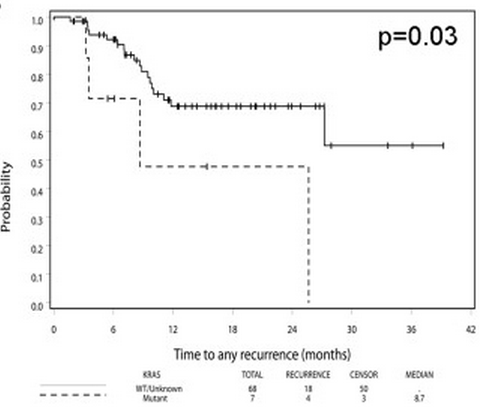
\includegraphics[width=0.6\textwidth]{kaplanmeier.png}
  \caption{\textbf{Time to recurrence}. Dotted line, K-Ras mutant, Solid line, K-Ras unknown or wild-type.\cite{mak2014}}
  \label{kaplanrecurrence}
  \end{figure}
  

  \subsection*{Ras functional biophysics}
  The Ras family proteins are small GTPases; that is, they are enzymes which can bind GTP and hydrolyze it to GDP, which remains bound until an exchange \cite{pyla}. In its GTP-bound form, Ras is active, and engages downstream pro-growth signaling factors as seen in \Cref{growthfig}. Ras is then inactivated by hydrolyzing its bound GTP; however, this process is greatly assisted by a family of proteins known as GTPase Activating Proteins, or GAPs \cite{pyla}. 
    \begin{figure}[H]
  \centering
  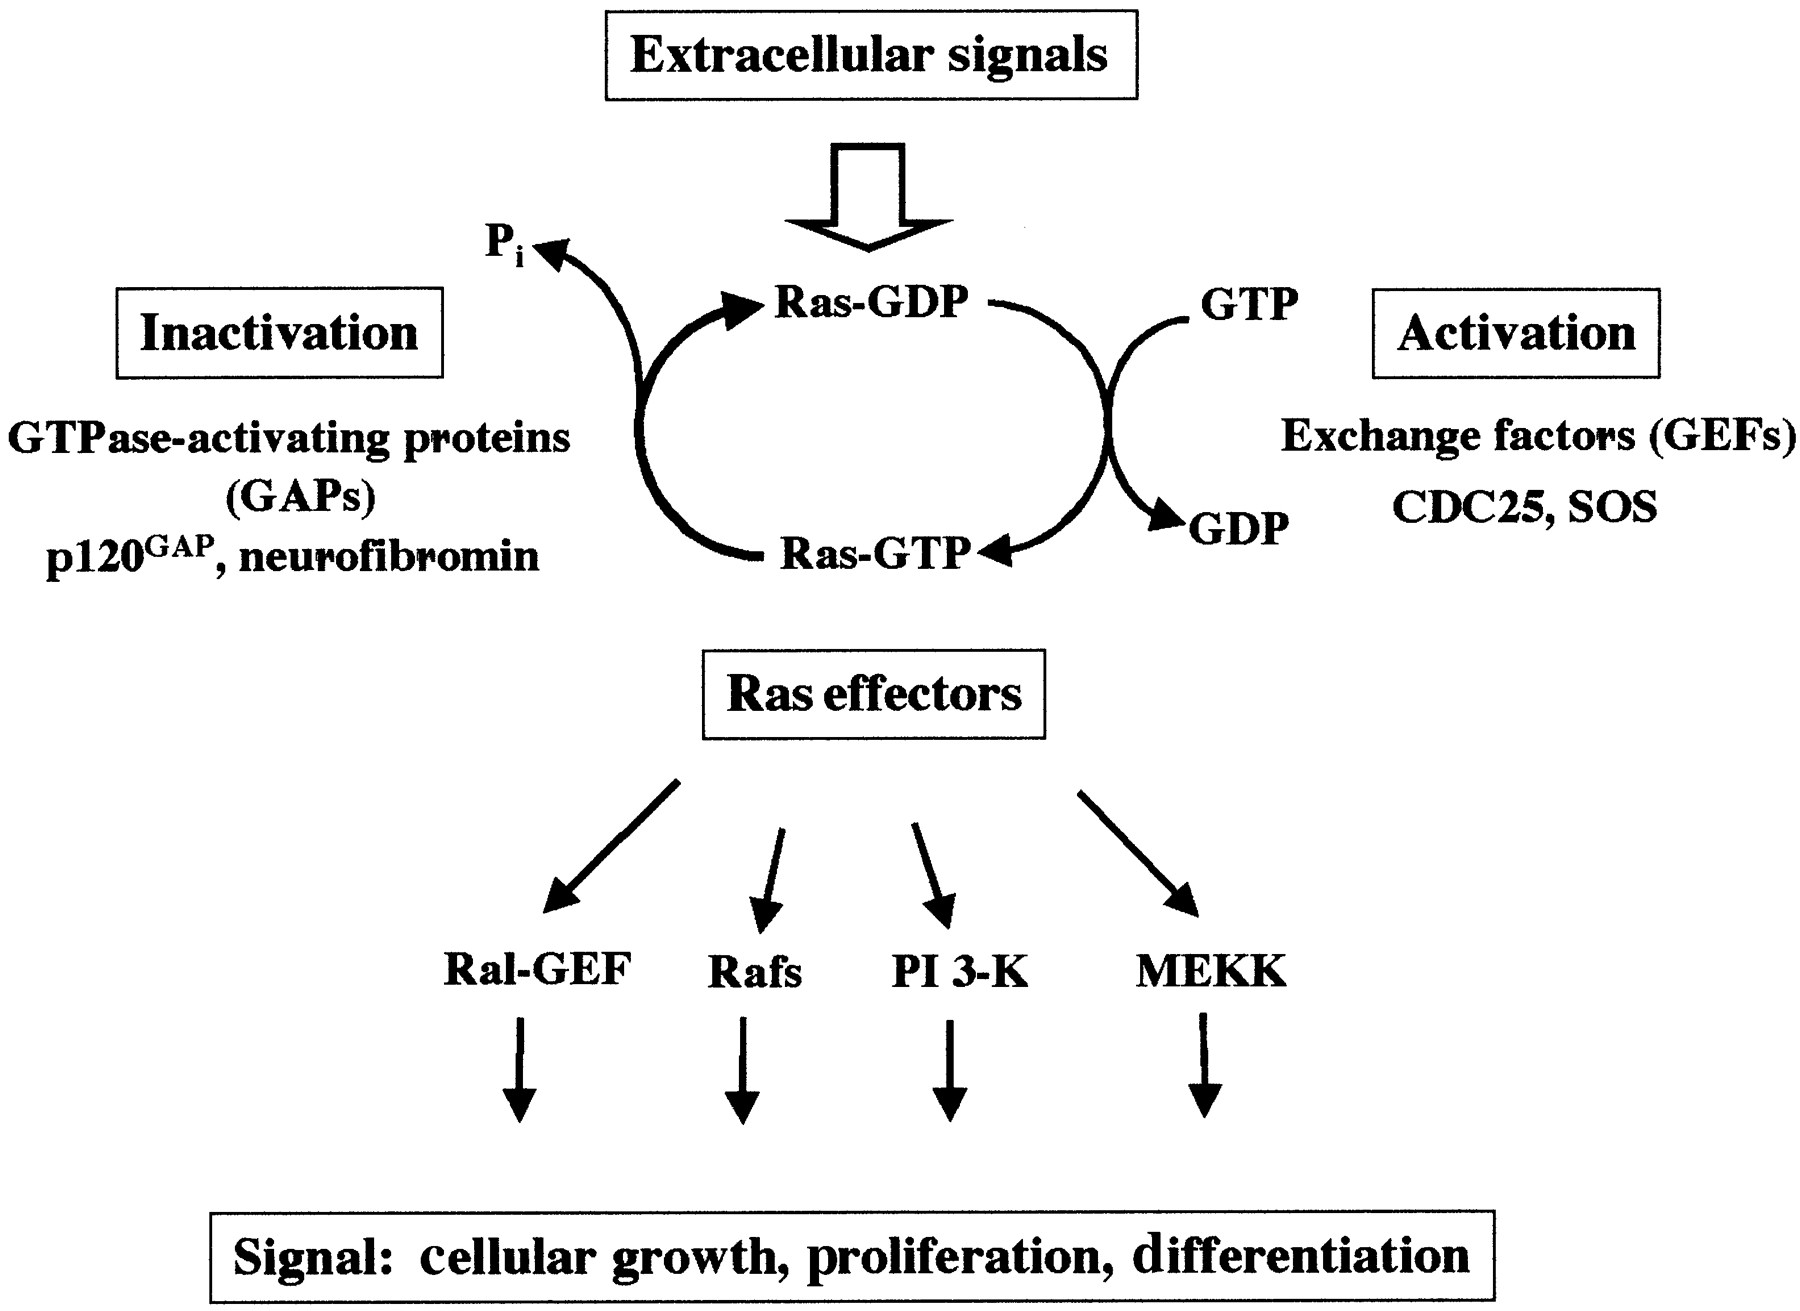
\includegraphics[width=0.6\textwidth]{ras_blood.jpg}
  \caption{\textbf{A diagram of major Ras growth signaling partners, indicating its connectedness in growth signaling pathways} \cite{rasblood}}
  \label{growthfig}
  \end{figure}
  The oncogenic potential of K-Ras mutations relates to its central role in cellular growth signaling \cite{pyla}, as indicated by \Cref{growthfig}. This position in relevant pathways makes Ras both a critical means of cancer proliferation and an attractive drug target. However, its biophysical nature causes great difficulty in designing an inhibitor; first, oncogenic mutations generally ablate the ability for Ras to hydrolyze GTP, as well as its ability to interact with partners that assist in hydrolysis and thus become inactive \cite{pyla}. This loss-of-function mutation means that inhibition of the enzymatic activity is not a feasible avenue. Furthermore, outcompeting bound GTP is generally regarded as infeasible due to its picomolar affinity for GTP \cite{ostrem2013} , and the lack of any other apparent  binding sites in crystal structures \cite{ostrem2013}.
  
  \section*{Approach}
  \subsection*{Aim 1: Computationally map conformations accessible to Ras along with their corresponding energetics to identify potential opportunities for allosteric modulation}
  
  \subsubsection*{Hypothesis}
  Ras family proteins can adopt multiple kinetically metastable states containing binding sites not present in the ground state, which can be observed using advanced molecular simulation techniques with the apo-protein.
  \subsubsection*{Overview:}
  As discussed above, Ras is a key protein in the ability for cancer cells to grow and divide, but the loss-of-function nature of its mutations and lack of apparent druggable sites render it a difficult target. While no apparent viable sites for ligand binding are present in crystal structures, there is evidence that there exist lower-populated conformations \cite{fesik} \cite{ostrem2013} which contain ligand binding sites, and may be signaling-inactive. However, the question remains of whether these sites, and potentially others, can be discovered in the absence of ligand. In order to answer this question, we will use parallel high-throughput molecular dynamics to generate trajectory data, and Markov State Modeling (MSM) \cite{chodera2014} to combine the trajectory data into a conformational map, as conceptually illustrated in \Cref{craikfig}.
  
    \begin{figure}[H]
  \centering
  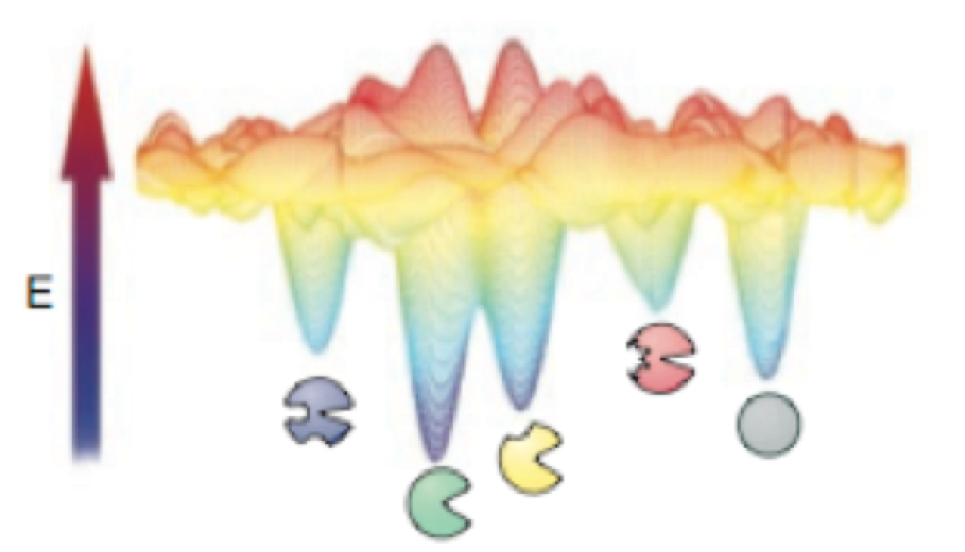
\includegraphics[width=0.5\textwidth]{craik.png}
  \caption{\textbf{A schematic of an energy landscape with multiple wells for metastable states} \cite{craik}}
  \label{craikfig}
  \end{figure}
  
  \subsubsection*{Aim 1.1: Identify metastable conformations and the associated energetics of oncogenic K-Ras using Markov State Model approaches}
   Here we propose to use parallel molecular dynamics simulations with OpenMM \cite{openmm}, and to combine the independent trajectories using Markov State Model approaches \cite{chodera2014} to elucidate the equilibrium conformational populations of oncogenic K-Ras and their interconversion kinetics. We also propose to use techniques developed in our laboratory to accelerate sampling, described below. The completion of this aim will not only render useful conformations for cancer drug discovery, but will also demonstrate that molecular dynamics can discover allosteric sites not visible in experimental structures, even in the absence of a ligand to stabilize those structures.
   
   \underline{Rationale:} As we would like to determine whether the conformational populations of K-Ras in detail we will use the computational technique of atomistic molecular dynamics. In using atomistic molecular dynamics to test our hypothesis, we are presented with several options. It may seem straightforward to simply run dynamics near an interesting conformation until binding sites appear. However, this suffers from the serious limitation that it does not provide equilibrium population data for an identified conformation. A more rigorous approach would involve running a single trajectory of a Ras protein for a very long time; however, this approach suffers from the practical limitation that it is difficult to take advantage of parallel computing resources. Instead, we propose to utilize the developing field of Markov State Modeling, which enables us to run many trajectories in parallel and distill trajectories into a set of kinetically metastable states with  \cite{chodera2014}, enabling us to achieve vastly greater sampling and take advantage of modern hardware such as Titan and Folding@Home.
  
 \underline{Specific Experiments:} In order to generate our conformational model via Markov State Modeling (MSM), we will first run many independent simulations of G12C-mutant apo K-Ras in explicit solvent, as this mutation is both clinically relevant and the subject of recent investigation \cite{ostrem2013}. We intend to repeat this protocol on other mutations and with GTP- and GDP-bound forms of K-Ras, allowing us to explore differences in equilibrium populations. To run the simulations, we will use Titan, a supercomputer at Oak Ridge National Laboratory and the second-fastest in the world.  To enhance sampling of conformational space, we will use a pipeline developed in our laboratory that identifies protein structures in the protein data bank (PDB) by BLAST \cite{blast} sequence similarity, then constructs homology models of the target sequence using MODELLER \cite{modeller}, followed by a brief molecular dynamics refinement as shown in \Cref{msmseeder}.  
 
 \underline{Data Analysis and Anticipated Results:} After trajectory data is collected, our first step in MSM creation will involve a dimensionality-reduction technique. This transforms input coordinates, such as distances or torsions, into a new, lower-dimensional, set of coordinates representing important (such as slowly-changing) features. Next, a technique such as Voronoi tessellation is used to assign the reduced-dimension trajectories to discrete states \cite{chodera2014}. These now-discretized trajectories are used to estimate the transition matrix between states \cite{chodera2014}. By using a maximally-connected subset of states in this final step, we can avoid the inclusion of potentially problematic simulations of irrelevant conformational states \cite{kyle}. The result of this process is a set of metastable conformations, along with transition probabilities between them, allowing us to examine the equilibrium conformational populations of K-Ras for ligand binding sites. We will verify that similar results are obtained using different subsets of the trajectory data, providing an indication that the conformational space of K-Ras has been sufficiently sampled. We expect that the conformations recovered in this process will include those identified in both inactive and active crystal structures, as well as a variety of intermediate states.
 %



  \begin{figure}[H]
    \centering
    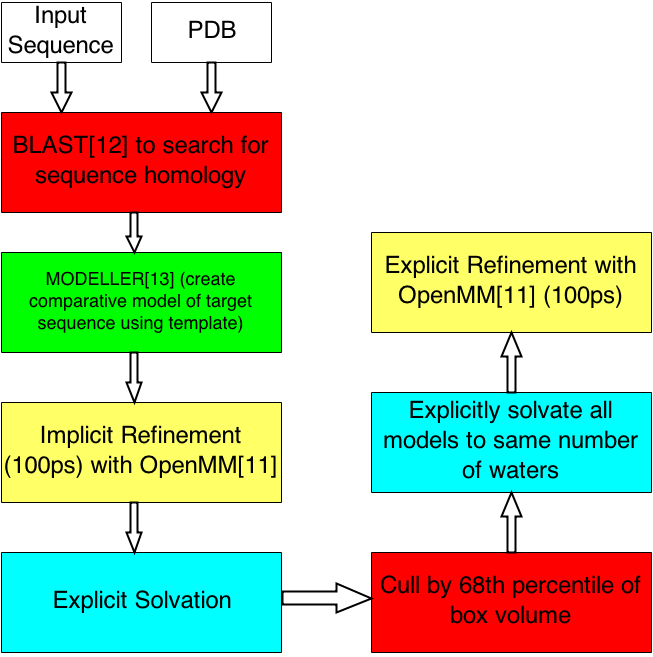
\includegraphics[width=0.5\textwidth]{msmseedernew_cite.png}
  \caption{\textbf{A flowchart demonstrating the generation of starting conformations.}}
  \label{msmseeder}
  \end{figure}
  
\underline{Potential Problems and Alternative Strategies:} While it is unlikely, it is possible that even given extensive sampling via supercomputers and from a diverse set of conformations, transitions between known relevant states of K-Ras will not be observed. In this event, we could further pursue techniques such as adaptive sampling \cite{chodera2014} to generate an MSM including transitions between known relevant states.
  
  \subsubsection*{Aim 1.2: Mine the Metastable Conformations for potential ligand binding sites}
  
  \underline{Rationale:} By generating an MSM of K-Ras, we are now afforded unprecedented insight into its equilibrium conformational populations. To test our hypothesis that this population, discovered without the presence of ligand, contains putative ligand binding sites, we intend to use an algorithm such as LIGSITE \cite{hendlich1997}. Furthermore, in order to identify potentially useful binding sites for drug discovery, we intend to use equilibrium population data to limit our selection of useful conformations to those which have an energy difference from ground that can be stabilized with a small molecule.\cite{kuntz1999}
  
  
  \underline{Specific Experiments and Data Analysis:} With our computational approach, we are afforded the opportunity to discover novel ligand binding sites that were not visible in experimental structures. We intend to screen the identified conformations with an algorithm known as LIGSITE \cite{hendlich1997}. This technique searches for points nearly-surrounded by solvent-inaccessible regions \cite{hendlich1997}. We believe that this will be successful for two reasons. First, this, approach has been used before to discover known cryptic binding sites in simulations without ligand \cite{bowman2012}. Second, the existence of weakly-binding molecules to allosteric sites on K-Ras, such as the covalent inhibitors in \cite{ostrem2013} depicted in \Cref{shokat_mols}, whose bound structure is illustrated in \Cref{shokatfig}. However, the molecules in \cite{ostrem2013} was discovered by a screening technique \cite{tethering} that requires covalent attachment, and still relies on serendipity. Our approach can discover allosteric sites without first requiring an allosteric ligand, allowing for rational allosteric drug design. Furthermore, in order to confine our identification of conformations with ligand binding sites to those which can conceivably be stabilized by a ligand, we will choose metastable conformations within 10$k_BT$ of the ground conformation \cite{kuntz1999}.
  
 \underline{Anticipated Results:} We expect that the analysis of metastable conformations will result in the identification of conformations with ligand binding sites, including those already discovered, despite the absence of ligand in the simulation. This provides us with several important pieces of information. First, it would confirm our hypothesis that the protein adopts these allosteric conformations even in the absence of ligand, albeit at a lower rate. Second, the result yields a structure to use for the discovery of novel ligands, which is not afforded by current experimental techniques.
 
 \underline{Potential Problems and Alternative Strategies:} It is possible that the MSM that we generated fails to generate novel allosteric binding sites. In this case, we will proceed with the proposal using already-identified sites. It is also possible that the MSM fails to identify pre-existing sites, though this seems highly unlikely. In that event, we will explore means to increase sampling, as well as run simulations including known ligands to test if they are required for appearance of the ligand binding site. 
  
  \begin{figure}[H]
  \centering
  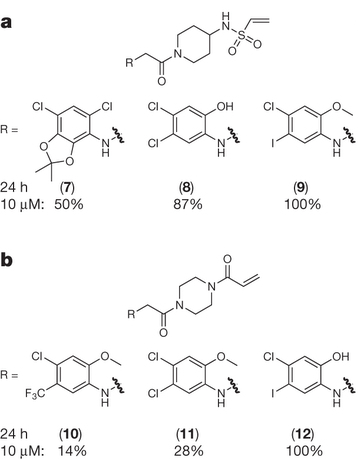
\includegraphics[width=0.4\textwidth]{shokat_mols.png}
  \caption{\textbf{Several molecules identified in \cite{ostrem2013} to inhibit K-Ras G12C.} Percentages denote covalent attachment after 24h in 10$\mu M$ compound. Note the presence of an electrophile for covalent attachment to the required cysteine. Image from \cite{ostrem2013}}
  \label{shokat_mols}
  \end{figure}
  
  \begin{figure}[H]
  \centering
  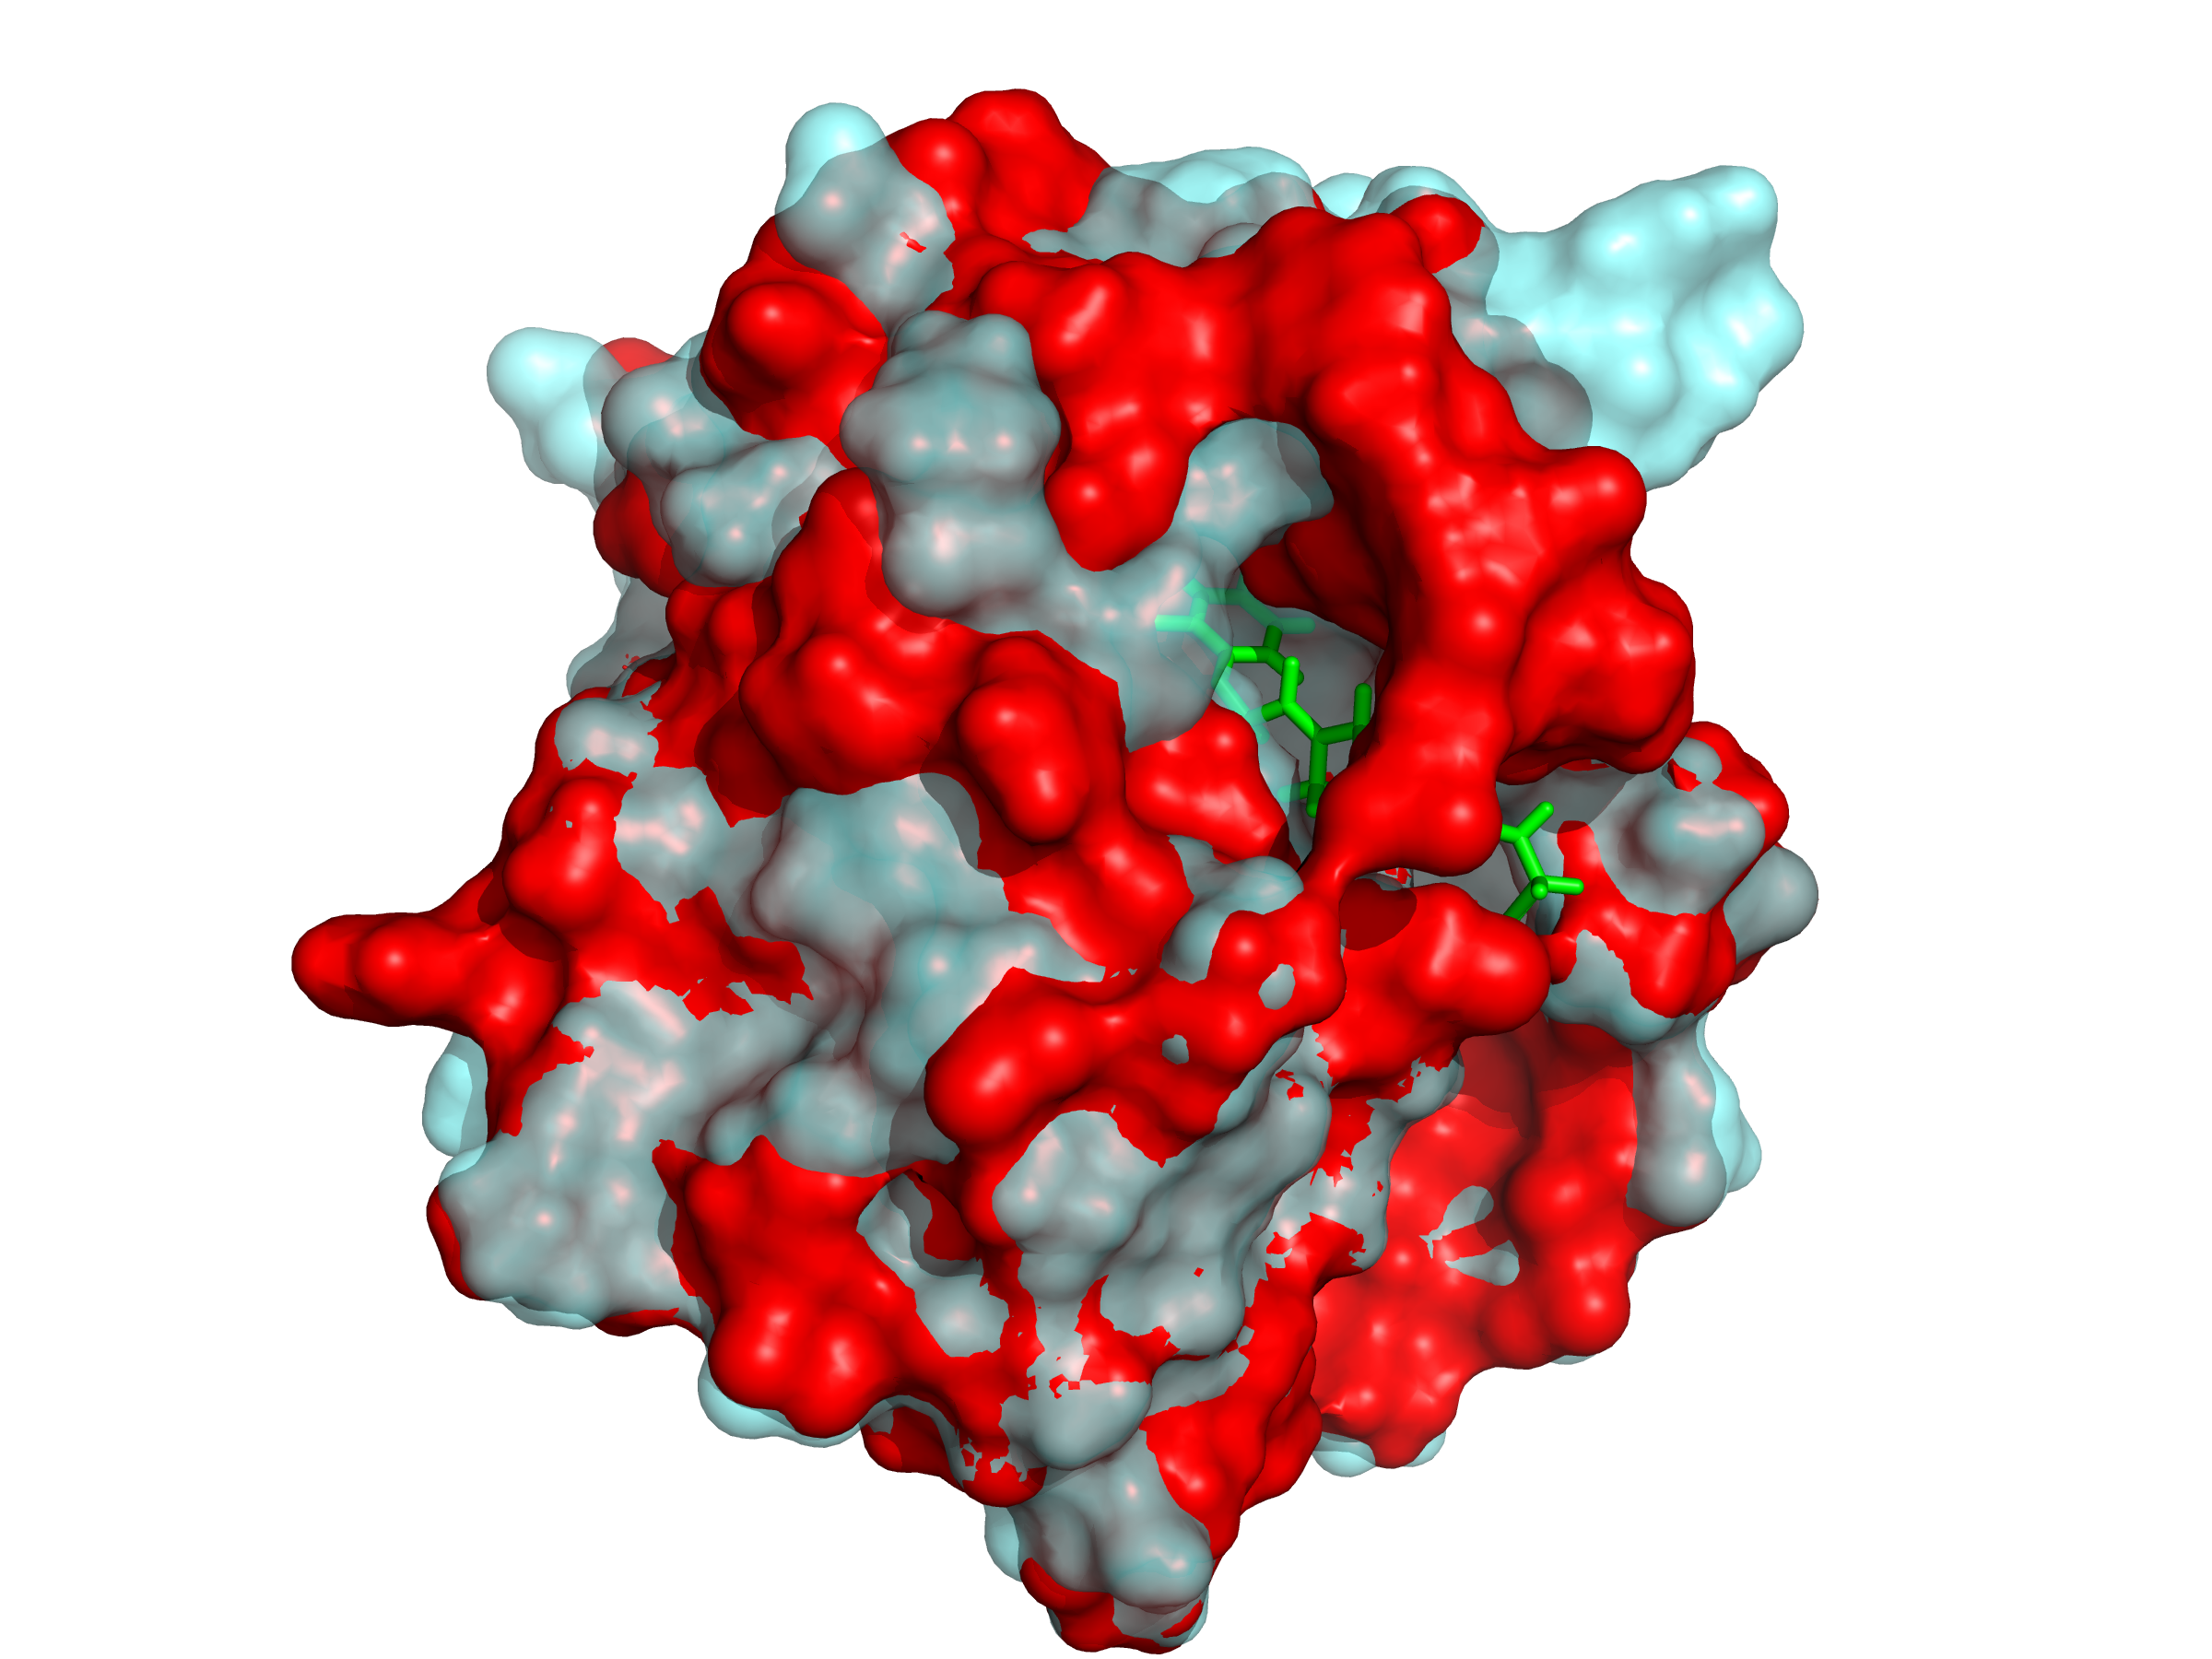
\includegraphics[width=0.8\textwidth]{ras_pocket.png}
  \caption{\textbf{K-Ras G12C (red surface) with bound inhibitor (green molecule), aligned to unbound structure (aquamarine surface)}. The ligand's presence reveals the presence of a binding pocket not visible in the unbound structure. \cite{ostrem2013}. PDB codes 4LV6 (bound) \cite{ostrem2013}, 4OBE (unbound) \cite{4OBEcite}.}
  \label{shokatfig}
  \end{figure} 

  \subsubsection*{Aim 1.3: Identify putative druggable signaling-inactive conformations} 
  
  \underline{Rationale:} Once we have identified metastable conformations, it is not only important to locate opportunities for ligand binding, but especially those states that may represent signaling-inactive states that could be preferentially stabilized by an allosteric ligand. The wealth of Ras structures bound to effectors as well as inactive will aid us in identifying conformations that may be unable to signal to downstream partners.
  
  \underline{Specific Experiments and Data Analysis:} Since the molecules in \Cref{shokat_mols} were shown to cause K-Ras to favor its guanosine diphosphate (GDP)-bound form instead of its active guanosine triphosphate (GTP)-bound form.\cite{ostrem2013}, it is plausible for us to search the metastable conformations for those with minimum RMSD to GDP-bound inactive structures. We will also examine the placement of nucleotide-interacting residues in identified metastable conformations and compare them to those of known GDP- and GTP-bound Ras structures. Additionally, we will examine structures involving key interaction partners of Ras. These proteins include SOS, an upstream effector that encourages nucleotide exchange, Raf, a group of protein kinases, and phosphoinositide 3-kinase (PI3K) \cite{pyla}. Comparison of available crystal structures of Ras-family proteins bound to these effectors with structures of inactive Ras can also lend insight into which conformational features are required for Ras activity \cite{pi3k}, such as those indicated in \Cref{raspi3kinteraction}. 
  \begin{figure}[H]
  \centering
  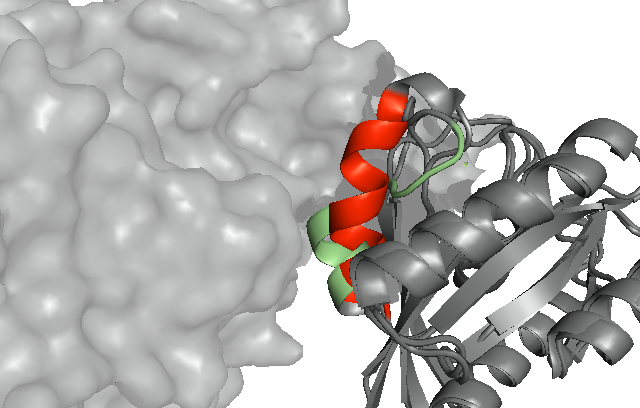
\includegraphics[width=0.5\textwidth]{new_ras_pi3k.png}
  \caption{\textbf{Alignment of GDP and GTP bound conformations of H-Ras, showing Switch II effector region interacting with Phosphoinositide 3-kinase $\mathbf{\gamma}$ (PI3K$\gamma$) \cite{pi3k}.} Red and aquamarine show active and inactive conformations, respectively, with PI3K$\gamma$ surface. PDB codes: inactive 1Q21 \cite{rasgdp}, active 1HE8 \cite{pi3k}}
  \label{raspi3kinteraction}
  \end{figure}
  
  \underline{Anticipated Results:} We expect that our analysis of the metastable conformations of Ras will include conformations in both active and inactive states. Furthermore, we expect that we will identify conformations with potential ligand binding sites that have key residues, as shown in \Cref{raspi3kinteraction}, in the inactive positions. This discovery of previously unknown inactive states would represent a number of important steps forward. First, it would further the understanding of how Ras functions, revealing novel metastable states and generating new hypotheses about the interaction of Ras with its effectors. Second, the discovery of metastable, inactive states with ligand binding sites would enable novel opportunities in the development of therapeutics targeted at Ras.
  
  \underline{Potential Problems and Alternative Approaches:} While we expect to recapitulate the inactive conformations of Ras, it is possible that we do not identify a conformation that is both inactive and exposes a ligand binding site. We find this to be highly unlikely, due to recent work \cite{ostrem2013} \cite{fesik} which give us confidence that such sites exist. However, a potentially more interesting problem is that a conformation identified as inactive is actually active, potentially signaling through a non-canonical effector. While our work could continue even in this case (as we use the previously-discovered structure in \cite{ostrem2013}), this finding would lead to an interesting avenue of research into a novel Ras signaling partner.
    
  \subsubsection*{Aim 1.4: Experimentally validate predicted conformational populations}
  
  \underline{Rationale:} Once we have constructed a computationally useful MSM of Ras, it is important to perform experiments to validate that we have actually modeled the system in a relevant manner. Therefore, we propose to perform experiments where we can measure observable quantities, such as a hydrogen-exchange protection factor, that we can also predict within our MSM. 

\underline{Specific Experiments and Data Analysis:} Given a set of metastable conformations and their relative equilibrium populations, we first propose to calculate a quantity known as the "protection factor" for each backbone amide hydrogen, such as is done in \cite{hx}. This quantity reflects the likelihood of a proton to exchange with protons in the solvent, and is directly related to solvent-accessibility as well as lack of intramolecular hydrogen bonding at that point. To measure the quantity experimentally, we propose an experiment known as hydrogen-deuterium exchange mass spectrometry (HDX-MS). In this experiment, the protein is exposed to heavy water, allowing protons in the protein to exchange with deuterons in the solvent. Then, the protein is analyzed by mass spectrometry for sites which have exchanged their protons with deuterons. Due to the high sensitivity of mass spectrometry, even relatively low populations can be detected via this method, using very little protein \cite{hdxms}. We will then compare the results of this experiment with the results of our calculations to validate that the MSM is accurately representing conformational populations of Ras. 

\underline{Anticipated Results:} We expect that the protection factors calculated from the MSM of K-Ras will match well with those measured by HDX-MS or NMR. Furthermore, we expect that the experiment will confirm the presence of existing and putative metastable binding sites, as a protection factor different from that expected from the crystal structure should be measured at those sites.

\underline{Potential Problems and Alternative Approaches:} While these experiments are demonstrated in other studies \cite{hdxms}, it is possible that we will find it difficult to obtain single-residue resolution using HDX-MS. In this case, we will turn to an established NMR technique for measurement of the same quantity. Alternatively, we could perform the NOESY experiment, which generates data that is related to the equilibrium distance between nuclei. 
  
  
  
\subsection*{Aim 2: Identify new small molecule ligands of Ras}
While screening can often identify weakly binding ligands, it is not typically clear where to proceed from there. We propose to develop a novel technique in which we can use the principles of statistical mechanics to derivatize ligands in a systematic way. We will develop an expanded-ensemble simulation that explores chemical space, allowing us to design ligands using principles of physics.

\subsubsection*{Hypothesis}
Certain chemotypes are more likely to be found at a particular binding site than others. Here, we ask the question of which chemotypes are necessary to bind to the allosteric sites identified in Aim 1 using a novel theoretical framework, presented below.

\subsubsection*{Aim 2.1: Perform virtual screening on a library of commercially-available compounds against putative allosteric binding sites}

\underline{Rationale:} Once we have identified suitable metastable conformations, we intend to begin a virtual screen with a large library of purchasable drug-like fragments. This will allow us to discover new scaffolds for allosteric Ras ligands, and is an important step in the direction of novel Ras inhibitor design, serving as a launching pad for our method for rational optimization.

\underline{Specific Experiments:} Databases such as ZINC \cite{irwin2012} can provide collections of molecules that are readily available for purchase and meet certain criteria. We intend to begin by virtual screening compounds in the "Frags now"  database, which is a database of over 1 million readily-available "fragment-like" (predicted logP$\leq$3.5, molecular weight$\leq$250, and the number of rotatable bonds$\leq$5). We will also filter by solubility, as the initial assays will take place at high concentration. The choice of the fragment database will allow us to screen a broad area of drug-like chemical space. We then intend to perform a docking-based virtual screen of our library against the conformations identified in Aim 1s, targeted at the potential binding sites for a small molecule. We will use a variety of docking tools to perform this screen after testing for known ligand binding over decoys. Molecular docking is a technique that uses a scoring function based on select features of the protein and ligand. While it often omits important features of the interaction, docking can be used to enrich a large library of compounds for potential hits. \cite{dockingrev}. 

\underline{Data Analysis and Validation:} Because docking is not typically able to produce an accurate binding affinity\cite{warren2006} we will use the more rigorous alchemical free energy calculations on the enriched set from docking. These methods create multiple systems which are alchemically modified; that is, the ligand and protein are decoupled to varying degrees, from completely interacting to completely non-interacting. Free energy differences, along with error estimates, are then calculated between each state\cite{boresch2013}. We also intend to experimentally test the affinity of the compounds identified after the filter. If the compound is predicted to affect GTP affinity, we will use the assay depicted in \Cref{gtpassay}. We will also create multiple tryptophan mutants of Ras. These mutants will each contain a single tryptophan that will provide a fluorescent reporter of the conformational state off K-Ras; when a ligand predicted to stabilize an alternate conformation is added, we would expect to see a shift in the fluorescence of tryptophan residues exposed to a different solvent environment. 

\begin{figure}
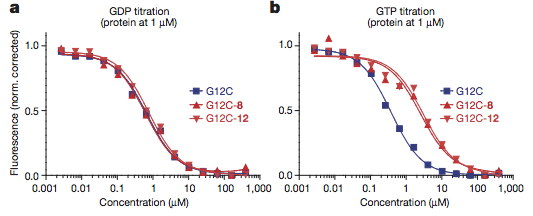
\includegraphics[width=\textwidth]{shokatassay.png}
\caption{\textbf{As demonstrated here, perturbation with a hit should result in a shift in the affinity for GTP} \cite{ostrem2013}}
\label{gtpassay}
\end{figure}

\underline{Anticipated Results:} Out of the large library of over 1,000,000 fragment-like molecules in the "frags now" database of ZINC \cite{irwin2012}, we expect docking to enrich a collection of molecules for fragments that will more likely bind to the predicted binding cavity. We further expect that that binding to sites exposed only in excited state conformations will perturb the equilibrium conformational populations of Ras in a ligand concentration-dependent manner. Finally, we expect that the results of this stage will be useful leads to pursue tighter-binding derivatives and a set of much-needed starting points for allosteric Ras modulators.

\underline{Potential Problems and Alternative Approaches:} While we expect that a large and diverse library will result in weak hits, it is possible that no such hits are present in the library. In this event, we could expand the library, or use a database of chemical transformations \cite{chemtransform} to expand the complexity of the libraries. Finally, if no compounds are discovered, we will proceed with the weak scaffolds discovered in \cite{ostrem2013} \cite{fesik}.

\subsubsection*{Aim 2.2: Perform Expanded Ensemble Simulations Over Chemical Space to Enhance Ligands}

\underline{Rationale:} Often, when hits are discovered, medicinal chemists use their chemical intuition and available chemistry to explore chemical space near the hit. However, this can be error-prone, time-consuming, and costly, especially as one realizes the combinatorial explosion of possible modifications of only a single hit. We propose instead to use a rigorous statistical mechanics framework to computationally explore the chemical space near derivatives of the scaffold to improve binding affinity. Using the theory of expanded ensemble simulation\cite{lyubartsev1992}, we will allow the lead to change various chemical substituents during simulation, biased toward tighter-binding ligands. 

\underline{Theory:}  As indicated in \Cref{markfig}, even a scaffold with four potential sites for modification and 10 modifications at each site can result in a search space of $10^4$ molecules. This is difficult both for traditional medicinal chemistry and for free energy calculations.  Therefore, to computationally explore this combinatorially large chemical space, we propose to use expanded ensemble simulation \cite{lyubartsev1992}, as described below.  We intend to use a database of chemical transformations, curated by medicinal chemists, to identify potential transformations of our ligand. These databases, such as \cite{chemtransform}, can allow us to propose changes to the ligand that are likely to be chemically accessible. 
\begin{figure}[H]
\centering
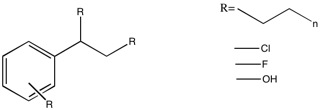
\includegraphics[scale=0.6]{cd_markush.jpg}
\caption{\textbf{An example of a Markush structure, containing combinatorially many possibilities.}}
\label{markfig}
\end{figure}
While simulation of biomolecules and ligands often proceeds via sampling (molecular dynamics or Markov Chain Monte Carlo) from the canonical ensemble, whose equilibrium distribution is given by \begin{equation} \pi(\textbf{x})=\frac{\exp[-u(\textbf{x})]}{\int \exp[-u(\textbf{x})] \mathrm{d}\textbf{x}}=Z^{-1}\exp[-u(\textbf{x})]\end{equation}
where \textit{u}(\textbf{x}) represents the reduced potential, given in its general form by

\begin{equation} \label{reducedu} u(\textbf{x})=\beta[U(\textbf{x})+pV(\textbf{x})] \end{equation}
where \textbf{x} is the configuration of the system, U(\textbf{x}) is the potential energy, V(\textbf{x}) is the volume (for a constant pressure simulation), p is the external pressure, and $\boldsymbol\mu$ is the chemical potential of each particle represented in \textbf{n}(\textbf{x}), which represents the number of particles in a (semi) grand canonical simulation \cite{shirts2008}. $Z$ represents the partition function, that is, the integral of $\exp[-u(\textbf{x})]$ over its entire domain. However, we need not restrict ourselves to this; we can define an \emph{expanded ensemble} such that we instead sample from a joint distribution given by \begin{equation} \label{eq:exens} \pi(\textbf{x},k)=\frac{\exp[-u_k(\textbf{x})+g_k]}{\sum_{i=1}^{k}\int \exp[-u_i(\textbf{x})+g_i] \mathrm{d}\textbf{x}} \end{equation} where the new parameter \textit{k} indexes the state of the simulation, and its corresponding $u_k$ gives the the reduced potential for that state and configuration. In our case, the state $k$ represents the current molecule, and a jump to a different state would represent a jump to a different ligand molecule. We also have the free parameter $g_k$, which enables us to weight each state with a biasing potential. Sampling from \Cref{eq:exens} often proceeds by Gibbs sampling \cite{liu}; that is, we draw a correlated sample from the conditional of \textbf{x} given \textit{k},
%
\begin{equation} \label{eq:xgivenk} \pi(\textbf{x}|k)=\frac{\exp[-u_k(\textbf{x})]}{\int \exp[-u_k(\textbf{x})] \mathrm{d}\textbf{x}} \end{equation}
%
followed by a sample from the conditional of \textit{k} given \textbf{x}:
%
\begin{equation} \label{eq:kgivenx} \pi(k|\textbf{x})=\frac{\exp[-u_k(\textbf{x})+g_k]}{\sum_{i=1}^{k}\exp[-u_i(\textbf{x})+g_i]} \end{equation}
%
To address the question of how to set the weights $g_k$, we will show that, for a specific convenient choice, the marginal distribution $\pi(k)$ is proportional to the binding affinity, $K_a$, such that the expanded ensemble simulation will be driven to spend more time in chemical states that are tighter binders.  This will enable expanded ensemble simulations to effectively hunt through large chemical spaces for good ligands. In order to derive this, we first marginalize out \textbf{x} in \Cref{eq:kgivenx}:
\begin{equation} \label{eq:marginalk} \pi(k)=\frac{\exp(g_k)\int \exp[-u_k(\textbf{x})] \mathrm{d}\textbf{x}}{\sum_{i=1}^{k}\int \exp[-u_i(\textbf{x})+g_i] \mathrm{d}\textbf{x}}\propto\exp(g_k)Z_{PL_k} \end{equation}

where $Z_{PL_k}$ represents the partition function for the protein-ligand complex \textit{k}.
We also know from thermodynamics that binding affinity, excluding multiplicative constants, is calculated as \cite{gilson1997}
\begin{equation} \label{eq:binding}K_a \equiv \frac{[PL]}{[P][L]} \propto \frac{Z_{PL}}{Z_{P\emptyset}} / \frac{Z_L}{Z_\emptyset} \end{equation}
%
and since the partition functions of the protein alone will not change during our expanded ensemble calculations, \Cref{eq:binding} is proportional to
%
\begin{equation} \label{eq:propbind} Z_{PL} /  \frac{Z_L}{Z_\emptyset} \end{equation}
%
Thus, setting the weight $g_k=-ln(Z_{L_k} / Z_\emptyset)$ yields an unnormalized probability for being in state \textit{k} of
%
\begin{equation} \label{eq:biasedk} \pi(k) \propto Z_{PL_k} / \frac{Z_{L_k}}{Z_\emptyset} \end{equation}
%
which is equivalent to the expression in \Cref{eq:propbind}. Therefore, by using a specific $g_k = -ln(Z_{L_k} / Z_\emptyset)$, we can steer the simulation toward molecules with better $K_{a}$ naturally. Though the above framework is theoretically sound, the presence of explicit waters near the site of transformation may create very low acceptance rates for state-change proposals, as there will likely be a clash if the ligand is instantaneously modified. We intend to take advantage of recent work \cite{nilmeier2011} that has shown that one can make nonequilibrium moves and preserve the equilibrium distribution. Using this scheme, we would not simply propose to instantaneously change the state, but rather propose a protocol to transition between the current state and the next proposed state, interleaving partial perturbation steps with propagation steps. The final move is then accepted or rejected based on the nonequilibrium work performed, and, to preserve the equilibrium distribution, momenta are reversed if the move is rejected. As shown in \Cref{ncmcfig}, for the test case of a WCA dimer, the use of NCMC dramatically increased acceptance rates and dramatically decreased correlation times.

\begin{figure}
\centering
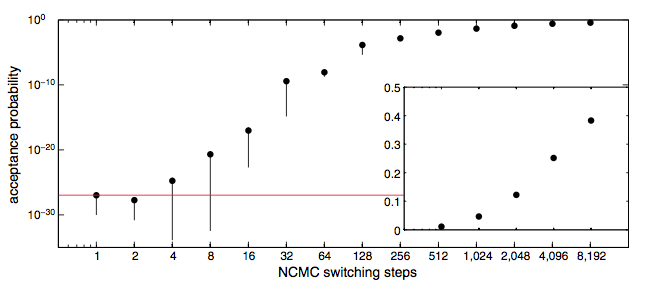
\includegraphics[width=0.6\textwidth]{ncmc.png}
\caption{\textbf{NCMC can improve the acceptance rates of MC moves (such as those that will be used to propose changes in chemical identities) by orders of magnitude.}\cite{nilmeier2011}}
\label{ncmcfig}
\end{figure}

\underline{Specific Experiments and Data Analysis:}  Although the above is tantalizing, calculating the normalizing constant of the ligand (equivalent to its hydration free energy) is nontrivial. Therefore, we propose to use single point energies, given by a simple evaluation of the forcefield at a minimized conformation in implicit solvent to provide an estimate for the weight to use in expanded ensemble simulation. This choice is considerably faster to evaluate, and, as we suggest below, may be a reasonable choice. We plan to run an expanded-ensemble simulation, starting from a weakly-binding ligand identified in Aim 2.1, using the aforementioned choice for the biasing potential. This choice is motivated by recent work \cite{mobley2008} indicating that though point energies of ligands may be insufficient for calculating hydration free energy estimates, they are relatively close (RMSE=0.39$\pm$0.05 kcal/mol for minimized ligands in solvent) \cite{mobley2008}. After running simulations, and binning the number of samples from each ligand, we will perform free energy calculations on the ligands that the simulation visited, and compare the rankings from the expanded ensemble to those of the free energy calculation.

\underline{Anticipated Results:} We expect that this theoretical result, and its practical application, will serve as a major innovation in drug design. Not only does it provide a method for enhancing ligand affinity that takes into account the dynamics of the protein and ligand, but it also allows us to ask questions about the nature of the relevant chemical space for binding a particular protein at a particular site, even in the absence of a ligand. We will use this information to interrogate identified Ras binding pockets for the relationship between chemotype and binding affinity. Additionally, because the single point estimates are relatively close to the hydration free energy values, we would expect them to still bias our expanded ensemble in the correct direction to discover tighter-binding ligands. Therefore, our free energy calculations should reflect a similar ranking as the expanded ensemble calculations. 

\underline{Potential Problems and Alternative Approaches:} Though previous results indicate that the point energy of minimized ligands is a good approximate to the hydration free energy, it is possible that, especially for larger and more flexible ligands, this approximation will not be appropriate. In this event, we could use hydration free energies to bias the simulation, as indicated in the theoretical result. Another potential issue is that the large number of low-affinity ligands that could be sampled will overwhelm the simulation, causing it to spend inordinate time sampling poorly-binding ligands. To remedy this, we will explore techniques to amplify the bias toward tightly-binding ligands.


\subsection*{Aim 2.3 Test whether compounds identified via the expanded-ensemble method will bind more tightly to oncogenic K-Ras and potentially disrupt its phenotype}

\underline{Rationale:} Once we have obtained simulation statistics in the expanded-ensemble technique described above, we will want to confirm that the identified molecules actually bind.

\underline{Specific Experiments and Data Analysis:} The first step in confirming that these ligands bind is to run alchemical free energy calculations on the top-scorers, confirming that they bind to a considerable enough degree to warrant synthesis and wet lab experimentation. This is done because free energies of binding can be computed much more precisely this way than looking at $-kT ln [\pi(k)]$ from the expanded ensemble simulation. If the ligands appear to be tightly-binding in calculation, we will have them synthesized by collaborators at the organic synthesis core for \textit{in vitro} testing. Then, we will use assays as described above to assay for GTP/GDP presence with the ligand, as well as solvent-exposed regions. We will also measure the affinity of the ligand using isothermal titration calorimetry (ITC), very popular and important in binding affinity measurement\cite{itcref}, for which our lab is developing novel techniques. If the ligand is experimentally confirmed to bind, we will then collaborate with cancer biologists to assay cell growth in the presence of the inhibitor, as shown in \cite{ostrem2013}. Finally, having shown that the ligand inhibits cancer cell growth, we will contact a structural biology collaborator at Stony Brook University to assist us in generating X-ray crystal or NMR evidence of the bound pose of the ligand and K-Ras.

\underline{Anticipated Results:} We expect that subjecting our lead compounds identified in the previous screen to our technique of expanded-ensemble simulation will identify derivatives that are both synthetically realistic and tighter binders. We anticipate that this result will also indicate novel chemical motifs that may be relevant in targeting Ras, and may suggest a general approach for identifying relevant chemical space for targeting a particular protein/binding pocket. We furthermore expect that the ligand will stabilize the expected conformation and cause measurable changes in the activity of Ras. This will help pave the way for the development of novel anticancer drugs targeting this heretofore very difficult-to-target protein.

\underline{Potential Problems and Alternative Approaches:} While we expect this aim to result in a tighter-binding ligand, there are some potential pitfalls. One issue is that the proposed changes to the ligand are very difficult or infeasible to make in the lab; while we expect our synthetic feasibility model to avoid this, if it does occur, we will restrict the modifications available to a particular lead based on a more detailed curation process.


\section*{Conclusion}
Once completed, our technique will have accomplished several innovations. First, we will have produced novel ligands that target and stabilize Ras family proteins, providing a new avenue for development of therapeutics targeting this "undruggable" target, including producing data that can produce a quantitative structure-activity relationship for Ras ligands. We will also have produced a map of the conformational populations of Ras, enabling further studies of its functional biophysics, critical to understanding the oncogenic potential of Ras. Furthermore, as our technique is a systematic one, it will serve as a template for the discovery of allosteric sites and ligands, as well as a rigorous technique for the improvement of scaffold binding in the face of combinatorially-large chemical space.

\clearpage

\bibliographystyle{unsrt}  
\bibliography{\jobname}  




\end{document}

